\chapter{Cloud and virtualization concepts}

\section{Introduction}
Virtualization is an attempt to trick the operating system into believing it is running directly on its own across the entire hardware of the device, while another operating system runs alongside it, also tricked. Virtualization is used in servers and workstations to run multiple operating systems on the same machine and connect them to each other via virtual networks (Software-Defined Networks) Figure[\ref{fig:virtualisation1}].

\begin{figure}
	\centering
	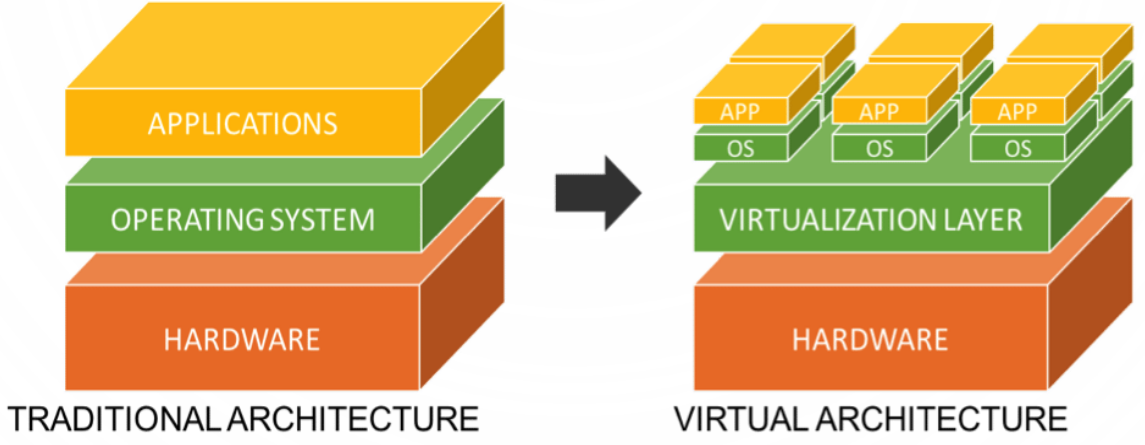
\includegraphics[width=0.7\linewidth]{figures/virtualisation1}
	\caption{virtualisation}
	\label{fig:virtualisation1}
\end{figure}

\section{Why we need virtualization}

\begin{itemize}
	\item Modern computing is more efficient due to virtualization
	\item Virtualization can be used for mobile, personal and cloud computing
	\item Virtualization enables computers to be more efficient in a similar fashion
	\item Computers that use virtualization optimize the available compute resources
\end{itemize}

\section{What is a Virtual Machine}
